\cleardoublepage
\chapter{Related Work}
\label{ch:relatedwork}
\label{ch:chapter2}

\section{Long-Context LLMs}

Various mechanisms have long been studied in Natural Language Processing for modeling long-term dependencies. Before the introduction of the transformer architecture, Recurrent Neural Networks (RNNs) represented the state-of-the-art language models. RNNs maintain a hidden state that recursively propagates through the sequence, allowing them to encode information from previous tokens as context for later inputs \cite{alma991005389998907681}. However, RNNs were not only prohibitively expensive to train but also difficult to optimize due to issues like vanishing and exploding gradients \cite{dai-etal-2019-transformer}.

\noindent Transformer-based architectures address many of these challenges by replacing recurrence with a self-attention mechanism, which allows each token to attend to all others in the input sequence \cite{10.5555/3295222.3295349}. This architecture has enabled the dramatic scaling of language models in recent years. Unfortunately, the self-attention block incurs a time and space complexity of $O(n^2)$ with respect to the sequence length $n$, making it costly to increase context window sizes with this approach alone \cite{pmlr-v201-duman-keles23a}\cite{wang2023augmentinglanguagemodelslongterm}. 

\noindent To mitigate this, some recent architectures have attempted to introduce recurrence into the transformer architecture, but these suffer from information loss over long sequences \cite{dai-etal-2019-transformer}. Other approaches, such as positional interpolation, attempt to rescale position indices to align with those used during pretraining. While effective in some cases, they are limited to RoPE-based LLMs, and certain configurations, such as static YARN,  have been shown to significantly degrade performance on shorter texts \cite{ding2024longrope}\cite{peng2024yarn}.
Alternative strategies include the use of external memory modules or residual side networks that persist information across inputs \cite{wang2023augmentinglanguagemodelslongterm}. However, these methods are still constrained by architecture-specific limitations.

\noindent While this area of research is promising, using the context window alone comes with significant challenges. First, embedding all information directly into the context window leads to increased token usage and higher computational cost. Second, as more content is added into the input, it becomes increasingly difficult for the model to effectively attend to the most relevant information, often resulting in reduced performance \cite{liu2023lostmiddlelanguagemodels}\cite{leng2024longcontextragperformance}.

\section{Retrieval Augmented Generation}

Retrieval Augmented Generation enhances LLMs by integrating relevant knowledge from external data sources into their context. Rather than relying on parametric memory, RAG retrieves supporting facts from separate knowledge sources, making it a widely used and cost-effective approach for providing accurate and up-to-date information to the model \cite{lewis2021retrievalaugmentedgenerationknowledgeintensivenlp}. Figure \ref{fig:rag} illustrates a common RAG pipeline used for a QA scenario.

\noindent Recent work has  extended RAG to support long-term memory in language agents by enabling them not only to retrieve from external stores but also to write new information to them \cite{Zhong_Guo_Gao_Ye_Wang_2024}.

\begin{figure}[h]
    \centering
    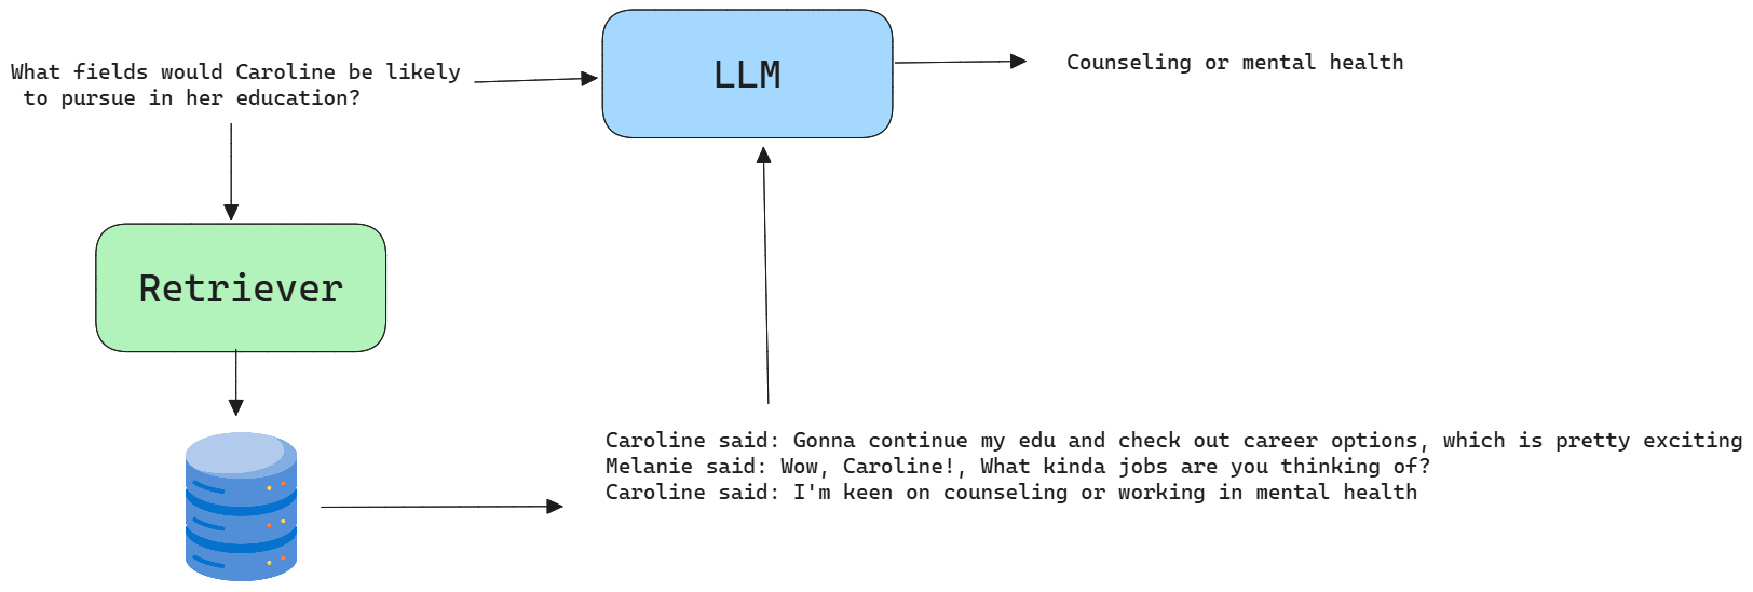
\includegraphics[width=0.95\textwidth]{images/rag.pdf}\\[-0.25cm]
    \caption{Illustration of a standard RAG pipeline. The input question is first processed by a retriever, which accesses an external document store to find relevant context. The retrieved information is then passed to an LLM that generates a final answer \cite{yaosu2024racm3}.}
    \label{fig:rag}
\end{figure}

\noindent Various studies have explored various retrieval granularities, including chunks, summaries, and knowledge triples \cite{zeng2024structuralmemoryllmagents}, as well as a range of retrieval algorithms, such as BM25 and semantic similarity methods.

\noindent Graph RAG extends this approach by using an LLM to extract entities and relationships from a corpus, constructing a knowledge graph that enables more effective reasoning over structured data. This structured representation is beneficial for answering global questions where conventional RAG methods often underperform \cite{edge2024localglobalgraphrag}. HippoRAG, inspired by neurobiological systems, adopts a similar graph-based design and has shown promising results \cite{NEURIPS2024_6ddc001d}.

\noindent Unfortunately, RAG alone has been proven insufficient for  tasks that demand more complex reasoning, such as MHQA. These tasks often require the integration of additional reasoning components to achieve strong performance.

\noindent Moreover, even when RAG inference is scaled by retrieving more information, performance often plateaus \cite{leng2024longcontextragperformance}. This suggests that retrieval alone is not always enough, reasoning capabilities must also evolve to handle the increasing complexity and volume of retrieved information.

\section{Prompt Engineering}

Numerous prompting methods have been developed to leverage the capabilities of LLMs, enabling them to reason over complex datasets. Techniques such as \textbf{Chain of thought (CoT)} and \textbf{Few-Shot Prompting} have demonstrated impressive results in tackling complex tasks, including mathematical reasoning \cite{wei2023chainofthoughtpromptingelicitsreasoning}.

\noindent Other prompting methods are designed to more directly integrate reasoning and interaction. \textbf{ReAct}, for instance, is a prompting framework that interleaves reasoning and action, and is widely used in language agents to aid them in decision-making \cite{yao2023react}\cite{language-agent-tutorial}.

\noindent For long documents, \textit{\textbf{PEARL}} (\textbf{P}lanning with \textbf{E}xecutable Actions for \textbf{R}easoning over \textbf{L}ong documents) introduces a multi-stage prompting method. First, the LLM is prompted to generate a list of actions that could help answer a question. Then, it formulates a plan to execute these actions. Finally, the LLM follows the plan to generate the final answer, using the output of each action to inform the next step, ultimately guiding the model to the final answer \cite{sun-etal-2024-pearl}. 

\noindent Similarly, \textit{\textbf{Iterative Demonstration-Based RAG}}, proposed by Yue et al, addresses complex queries by decomposing them into simpler sub-queries. RAG is then applied to each subquery independently, leading to improved performance over single-pass RAG methods \cite{yue2024inferencescalinglongcontextretrieval}.

\noindent Further exploration of how various prompting methods can be effectively integrated with language agents remains a fascinating area of research \cite{trivedi-etal-2023-interleaving}. Understanding how these methods scale and interact with different RAG strategies is crucial for advancing the capabilities of language agents in handling complex reasoning and planning \cite{language-agent-tutorial}.

\section{Language Agents}

Language Agents refer to autonomous systems that integrate LLMs for reasoning and communication, using language as their primary means of interaction with the environment and decision-making \cite{language-agent-tutorial}. Figure \ref{fig:cognitive-arch} provides a high-level overview of the cognitive architecture behind these systems.

\noindent A key component of such agents is memory, which serves as an internal mechanism for storing and retrieving past information. This capability enables the agent to learn from experience, maintain coherence over long interactions, and make informed decisions. Examples of language agents that incorporate these concepts include MemGPT and Graph Reader, each adapted to different use cases and environments \cite{packer2024memgptllmsoperatingsystems}\cite{li2024graphreaderbuildinggraphbasedagent}.

\noindent Drawing inspiration from human cognition, memory in language agents can be categorized into four types: episodic memory, which stores experiences; semantic memory, which stores knowledge or facts; procedural memory, which captures skills or routines \cite{sumers2024cognitive}, and working memory, which handles short-term relevant information. 

\noindent Some systems, such as AriGraph, integrate episodic and semantic memories within a knowledge graph, allowing the agent to access and leverage structured information to apply it in complex reasoning tasks \cite{anokhin2024arigraphlearningknowledgegraph}.

\begin{figure}[h]
    \centering
    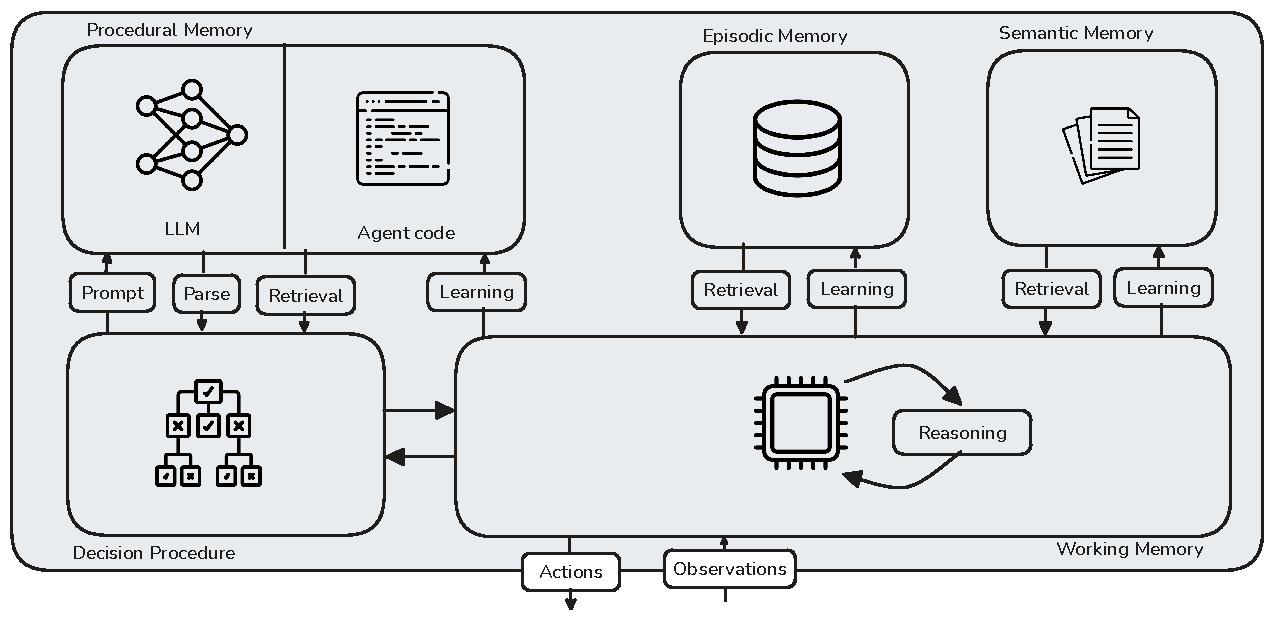
\includegraphics[width=0.95\textwidth]{images/cognitive-arch.pdf}\\[-0.25cm]
    \caption{Cognitive architectures for language agents \cite{sumers2024cognitive}.}
    \label{fig:cognitive-arch}
\end{figure}

\noindent Language agents can also be augmented with tools that extend their ability to interact with the environment. LLMs' capacity to process and generate structured data formats like JSON or XML enables integration with domain-specific APIs and external databases \cite{language-agent-tutorial}. AriGraph, for instance, uses this capability to navigate a knowledge graph and retrieve relevant information for QA tasks \cite{anokhin2024arigraphlearningknowledgegraph}.

\noindent The reasoning and planning capabilities of language agents become particularly relevant when combined with prompting strategies designed to guide multi-step thinking. Techniques, such as ReAct \cite{yao2023react}, help agents analyze their environment, make observations, and execute plans.

\noindent Recent work has also explored multi-agent systems, where language agents collaborate or debate to solve a task \cite{language-agent-tutorial}. For example, Zhao et al. introduced a collaborative framework for QA over long documents in which a leader agent partitions the document into $m$ chunks, delegates each to an agent, and then aggregates their responses. This iterative process continues until the leader agent determines a confident answer can be given \cite{zhao-etal-2024-longagent}.

\noindent Although language agents have been studied in a variety of settings, including text-based games, human simulacra, and task automation \cite{10.1145/3586183.3606763}\cite{anokhin2024arigraphlearningknowledgegraph}, questions remain about their role in natural language tasks such as QA and MHQA. In particular, further exploration is needed to understand how planning, collaboration, and memory, when combined with techniques like RAG and prompt engineering, can contribute to more effective and adaptable systems in these domains.


\section{Question Answering}

Question Answering (QA) is a foundational task in natural language processing that involves predicting an answer given a question and some context. Recent advances in LLMs have led to significant progress in this area, enabling the development of systems that perform well across a range of diverse datasets and domains \cite{10.1561/1500000102}.


\noindent Despite these improvements, certain QA sub-tasks remain challenging. For instance, Textbook Question Answering (TQA) poses difficulties due to its reliance on long passages, as well as the integration of visual elements such as diagrams and tables \cite{ALAWWAD2025111332}.

\noindent Another challenging variant is Multi-Hop Question Answering (MHQA), where answering a question requires combining information from multiple sources or passages. Unlike single-hop QA, where a single context snippet typically contains the answer, MHQA requires reasoning over multiple facts or steps to arrive at a correct response \cite{10.1561/1500000102}. See Table \ref{tab:questions} for various examples of MHQA questions.

\begin{table}[h]
    \centering
    \small
    \begin{tabular}{
        >{\raggedright\arraybackslash}p{2cm}  % Question Type
        >{\raggedright\arraybackslash}p{3.2cm}  % Question
        >{\raggedright\arraybackslash}p{4.8cm}  % Context
        >{\raggedright\arraybackslash}p{1.6cm}    % Answer
    }
        \toprule
        \textbf{\scriptsize Question Type} &
        \textbf{\scriptsize Question} &
        \textbf{\scriptsize Context} &
        \textbf{\scriptsize Answer} \\
        \midrule
        Comparison & Which film came out first, Blind Shaft or The Mask Of Fu Manchu? & 
        Blind Shaft is a 2003 film about a pair of brutal con artists \ldots\par\vspace{.5\baselineskip}
        The Mask of Fu Manchu is a 1932 pre-Code adventure film directed by Charles \ldots\par\vspace{.5\baselineskip} & 
        The Mask Of Fu Manchu \\

        Compositional & What is the place of birth of the director of film Deadbolt (Film)? & 
        Deadbolt is a 1992 made-for-television thriller film, by Douglas Jackson, and starring Justine Bateman, Adam Baldwin, and Michele Scarabelli \ldots\par\vspace{.5\baselineskip}
        Douglas Jackson (born January 26, 1940 in Montreal, Quebec) is a Canadian film and \ldots\par\vspace{.5\baselineskip} & 
        Montreal, Quebec \\

        Compositional & How many miles is Sloan Thomas' birthplace from Nashville? & 
        Sloan Thomas (born December 22, 1981 in Clarksville, Tennessee) is a former American football wide receiver from the National Football \ldots\par\vspace{.5\baselineskip}
        The city of Clarksville is a fifth significant population center, some 45 miles (72 km) northwest of Nashville \ldots\ & 
        45 \\
        \bottomrule
    \end{tabular}
    \caption{\small Examples of Multi-Hop questions taken from MuSiQue and 2Wiki \cite{trivedi2021musique}\cite{ho-etal-2020-constructing}.}
    \label{tab:questions}
\end{table}



\section{Evaluation Metrics}

To evaluate the performance of the cognitive language agents and baselines, we use a set of commonly adopted metrics for QA.

\begin{description}
    \item[Exact Match (EM)] Assigns a score of 1 if the predicted answer exactly matches the reference. EM is a strict metric and may assign low scores to answers that are semantically equivalent. Regardless, it is widely used in QA tasks \cite{tang-etal-2021-multi}.
    \item[ROUGE] Suite of metrics originally developed to evaluate the quality of automatically generated text, particularly in machine translation and summarization tasks. Among the many ROUGE variants, we focus on ROUGE-1 ($R_1$) and ROUGE-2 ($R_2$), which compute the harmonic mean of precision and recall over unigram and bigram overlaps, respectively, permitting duplicate n-grams \cite{lin-2004-rouge}. For predictions that are empty, often a result of model safety filters, we assign scores of 0 to both $R_1$ and $R_2$. Importantly, our use of $R_1$ is equivalent to $F1$ as typically used in the literature, with a small constant $\epsilon=1 \times 10^{-8}$ added to avoid division by zero \cite{mrqa-2021-machine}.
    \par
    \begin{equation}
        \text{ROUGE} = 2 \cdot \frac{\text{Precision} \cdot \text{Recall}}{\text{Precision} + \text{Recall} + \epsilon}
    \end{equation}
    \item[LLM Judge ($L_1$)] Human evaluation is a reliable method for assessing the quality of LLM-generated responses. However, it is both costly and time-consuming. Recently, LLM-based evaluators have gained popularity as a scalable alternative due to their ability to align well with human preferences \cite{zheng2023judgingllmasajudgemtbenchchatbot}. In our evaluation, we use an LLM judge as a binary evaluator \cite{li2024llmsasjudgescomprehensivesurveyllmbased}, which assigns a score of 1 if it determines that the predicted and reference answers are semantically equivalent. The increasing adoption of LLM-based judges reflects their ability to approximate human judgment at scale.
\end{description}

\noindent We place particular emphasis on $R_1$ and $L_1$, as they offer greater flexibility in recognizing semantically correct answers, even when the model deviates from the instruction to quote directly from the retrieved passages.

\noindent While other evaluation metrics such as BERTScore exist \cite{zhang2020bertscoreevaluatingtextgeneration}, we exclude them from our analysis due to the nature of our datasets, which primarily consist of conversational exchanges or Wikipedia passages. Many questions focus on specific entities, and semantic similarity metrics like BERTScore can produce misleadingly high scores for incorrect answers when the entities are close in the embedding space. Although research into alternative evaluation metrics for QA is ongoing, our chosen metrics are consistent with prior work and are well-suited to the datasets used in this study \cite{chen-etal-2019-evaluating}.
